
\begin{problem}
	You are given two bipartite graphs $G$ and $H$ below. For each
	graph determine whether it has a perfect matching.
	Justify your answer, either by 
	listing the edges that are in the matching or using
	Hall's Theorem to show that the graph does not have a
	perfect matching.

	\begin{center}
	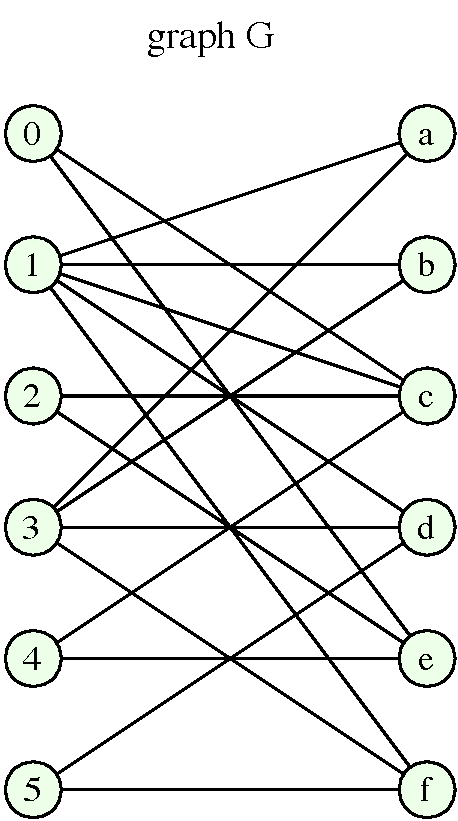
\includegraphics[width = 1.75in]{bipartite_graphG_hw5.pdf}
	\ \ \ \ \
	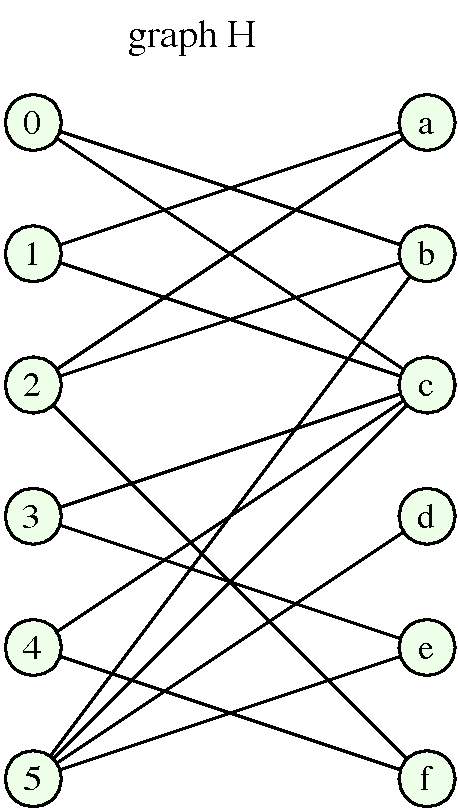
\includegraphics[width = 1.75in]{bipartite_graphH_hw5.pdf}
	\end{center}
\end{problem}

\begin{solution}
  Graph $G$ can be shown to not have a perfect matching.

	\begin{center}
	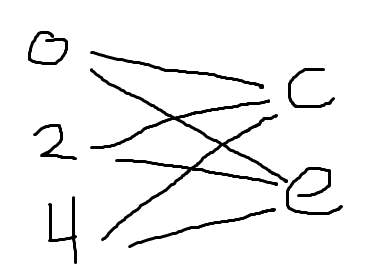
\includegraphics{big.png}
	\end{center}

  Observe that $For A \subseteq V_1, |A| > |Adj(A)|$. By Hall's Theorem, this shows there can be no perfect matching for $G$.

\bigskip

A perfect matching of graph $H$ is as follows

	\begin{center}
	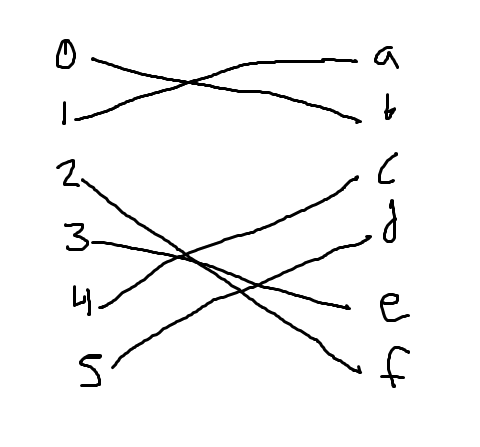
\includegraphics{bih.png}
	\end{center}

All vertices have one edge, so this represents a perfect matching of $H$
\end{solution}

%%%%%%%%%%%%%%%%%%%%%%%%%%%%

% new


